\chapter{METODE PENELITIAN}

\section{Waktu dan Tempat Pelaksanaan Penelitian}
Penelitian ini dilaksanakan pada bulan Januari hingga Februari 2026 di Laboratorium Program Studi Teknologi Mekatronika, Politeknik Enjinering Indorama (PEI), Kabupaten Purwakarta, Jawa Barat.

\section{Alat dan Bahan}
Adapun rincian spesifikasi serta kuantitas alat dan bahan yang digunakan pada penelitian ini disajikan pada Tabel \ref{tab:alat_bahan}.

\begin{table}[htbp]
\centering
\caption{Alat dan Bahan}
\label{tab:alat_bahan}
\begin{tabular}{|c|p{8.5cm}|c|}
\hline
\textbf{No.} & \multicolumn{1}{c|}{\textbf{Alat dan Bahan}} & \textbf{Jumlah} \\ \hline
1. & Laptop & 1 buah \\ \hline
2. & Raspberry Pi 5 & 1 buah \\ \hline
3. & Lengan Robot Dobot Magician & 1 buah \\ \hline
4. & Lengan Robot meArm (4-DOF) & 1 buah \\ \hline
5. & Kamera Web (Webcam) Logitech [Model: C270/HD] \newline (Resolusi: 640$\times$480 piksel, 30 FPS) & 1 buah \\ \hline
6. & Monitor Raspberry Pi & 1 buah \\ \hline
7. & Adaptor Daya (\textit{Power Supply}) Raspberry Pi & 1 buah \\ \hline
8. & \textit{Power Supply} 5V DC (untuk meArm) & 1 buah \\ \hline
9. & Papan Rangkaian (\textit{Breadboard}) & 1 buah \\ \hline
10. & Kabel \textit{Jumper} (\textit{Male-to-Male}/\textit{Male-to-Female}) & Secukupnya \\ \hline
11. & Kabel USB Serial & 1 buah \\ \hline
12. & Software Python 3.9 & - \\ \hline
13. & Pustaka Python: OpenCV (v4.9.0.80), MediaPipe (v0.9.0.1), TensorFlow/Keras, NumPy (v1.23.5), Protobuf (v3.20.3), Pydobotplus, PySerial, Tkinter, dan Pillow (PIL) & - \\ \hline
\end{tabular}
\end{table}

\section{Diagram Alir}
Adapun diagram alir penelitian ini adalah sebagai berikut.

\begin{figure}[htbp]
\centering
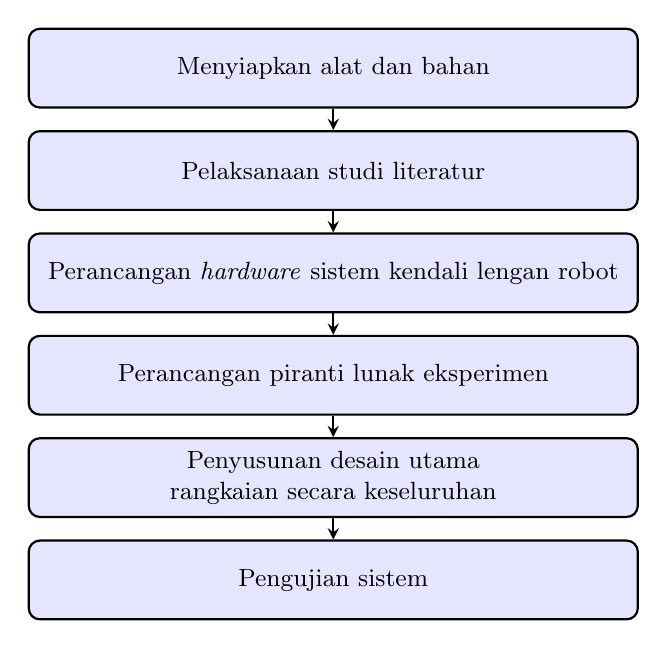
\begin{tikzpicture}[
    node distance=1.3cm,
    every node/.style={fill=white, font=\small},
    block/.style={rectangle, draw=black, rounded corners, fill=blue!10, text width=7.5cm, text centered, minimum height=1cm, line width=0.8pt},
    arrow/.style={thick, ->, >=stealth}
]
    \node (step1) [block] {Menyiapkan alat dan bahan};
    \node (step2) [block, below of=step1] {Pelaksanaan studi literatur};
    \node (step3) [block, below of=step2] {Perancangan \textit{hardware} sistem kendali lengan robot};
    \node (step4) [block, below of=step3] {Perancangan piranti lunak eksperimen};
    \node (step5) [block, below of=step4] {Penyusunan desain utama rangkaian secara keseluruhan};
    \node (step6) [block, below of=step5] {Pengujian sistem};

    \draw [arrow] (step1) -- (step2);
    \draw [arrow] (step2) -- (step3);
    \draw [arrow] (step3) -- (step4);
    \draw [arrow] (step4) -- (step5);
    \draw [arrow] (step5) -- (step6);
\end{tikzpicture}
\caption{Diagram Alir Penelitian}
\label{fig:diagram_alir}
\end{figure}

Penelitian ini diinisiasi dengan melaksanakan riset terkait studi literatur dari diversifikasi sumber yang teruji validitasnya. Riset ini dilakukan untuk menganalisis secara mendalam terkait landasan teori dari topik yang diteliti, menganalisis prinsip dan langkah kerja dari eksperimen yang dilakukan, dan memahami prinsip kerja dari alat yang digunakan dalam menunjang efektivitas eksperimen. Setelah dilaksanakan riset studi literatur, tahapan selanjutnya adalah perancangan \textit{hardware} dari sistem kendali lengan robot, mencakup di dalamnya pemilihan komponen dan memahami prinsip kerja, \textit{datasheet}, dan alur rangkaian dari purwarupa yang disusun.

Langkah selanjutnya setelah rangkaian berjalan dengan baik, tahapan yang dilakukan adalah menyusun piranti lunak, mencakup di dalamnya kode program terkait ekstraksi \textit{landmark} pengenalan SIBI dan algoritma kinematika, serta program antarmuka menggunakan piranti Python 3.9. Tahapan yang ditempuh setelah rangkaian \textit{hardware} dan tampilan antarmuka berjalan dengan baik dan konsisten, maka tahapan yang dilaksanakan adalah penyusunan desain utama rangkaian secara keseluruhan. Setelah seluruh tahapan dilakukan, maka tahapan akhir yang ditempuh adalah pengujian sistem secara keseluruhan. Tahapan ini mencakup di dalamnya pengukuran data dan pengolahan data serta membandingkan hasil yang diperoleh dengan referensi yang ada untuk memvalidasi efektivitas sistem.

\subsection{Studi Literatur}
Studi literatur yang ditempuh adalah menggunakan referensi yang kredibel, mencakup di dalamnya yaitu referensi berdasarkan jurnal terakreditasi, buku, dan dokumen resmi terkait prinsip kerja dari komponen yang digunakan. Literatur ini mencakup di dalamnya terkait teori yang mendasari ekstraksi \textit{landmark} MediaPipe, prosedur kerja eksperimen yang ditempuh, prinsip kerja dari aktuator lengan robot, prosedur kerja dari persamaan trigonometri \textit{Inverse Kinematics} yang disusun, pemodelan jaringan \textit{Deep Neural Networks} (DNN), dan tahapan pengukuran maupun pengolahan data yang dilakukan.

\subsection{Perancangan \textit{Hardware} Sistem Kendali Robot}
Pada tahap ini, tahapan prosedur difokuskan dalam penyusunan rangkaian secara elektronika. Penyusunan rangkaian dimulai dari penempatan aktuator Dobot Magician dan perakitan mekanis lengan robot meArm, yang keduanya diintegrasikan dengan modul Raspberry Pi 5 sebagai \textit{edge computer} utama yang terhubung ke Monitor Raspberry Pi. Kemudian, penyusunan rangkaian turut dilaksanakan dengan menghubungkan beberapa pin utama yang menghubungkan aktuator servo meArm terhadap pin GPIO mikrokontroler melalui bantuan \textit{breadboard} dan kabel \textit{jumper}.

Adaptor daya kustom dialokasikan khusus untuk menyuplai daya komputasi Raspberry Pi 5 agar tidak mengalami \textit{under-voltage}, sedangkan \textit{power supply} 5V DC eksternal digunakan untuk menyuplai arus penggerak motor servo meArm secara terpisah agar sistem terhindar dari gangguan \textit{noise} induksi motor. Kabel USB Serial juga dipasangkan secara fisik untuk menjamin kestabilan transmisi instruksi sudut dan koordinat dari port USB Raspberry Pi 5 menuju \textit{internal controller} Dobot Magician.

\subsection{Perancangan Piranti Lunak}
Tahapan perancangan piranti lunak mencakup penyusunan arsitektur pemrograman berbasis Python 3.9 yang mengintegrasikan pemrosesan citra, ekstraksi fitur penanda geometris, klasifikasi kecerdasan buatan, manajemen antarmuka grafis (\textit{Graphical User Interface}), dan komunikasi serial. Secara teknis, fungsionalitas piranti lunak ini dirancang menggunakan kontribusi dari beberapa pustaka utama dengan mekanisme kerja sebagai berikut:

Dalam inisialisasi awal program, sistem meluncurkan antarmuka pengguna grafis (GUI) yang dibangun menggunakan pustaka Tkinter. GUI ini memfasilitasi interaksi pengguna untuk memantau konektivitas robot, mengelola \textit{jogging} secara manual, serta memvisualisasikan mode kendali berbasis AI. Sementara itu, pustaka OpenCV (v4.9.0.80) dikonfigurasi untuk membuka saluran komunikasi visual dengan \textit{webcam} Logitech. OpenCV bertugas melakukan akuisisi bingkai (\textit{frame}) video secara \textit{real-time}, membalikkan citra secara horizontal (\textit{mirroring}), serta melakukan konversi ruang warna dari BGR ke RGB. Agar aliran citra visual tersebut dapat dirender dan ditanamkan (\textit{embedded}) ke dalam kanvas antarmuka Tkinter, program memanfaatkan pustaka Pillow (PIL) untuk mengonversi matriks array NumPy menjadi objek gambar (ImageTk) yang kompatibel dengan komponen GUI.

Setelah citra RGB diperoleh, data diumpankan secara langsung ke dalam kerangka kerja MediaPipe (v0.9.0.1). Di dalam struktur perulangan (\textit{main loop}), MediaPipe mengeksekusi model deteksi untuk mengekstrak 21 titik persendian spasial (\textit{landmarks}) dalam koordinat tiga dimensi $(x,y,z)$. Koordinat ini kemudian didistribusikan ke dalam dua logika kondisional berdasarkan mode operasi robot:

\begin{enumerate}[label=\arabic*.]
    \item \textbf{Alur Kerja Mode SIBI (meArm)}: Matriks koordinat 21 persendian tangan ditransformasikan ke dalam larik 1D dan dinormalisasi terhadap titik pergelangan (\textit{wrist}). Vektor fitur spasial yang telah siap kemudian diumpankan maju (\textit{feed-forward}) ke dalam model \textit{Deep Neural Networks} (DNN) yang dimuat menggunakan pustaka TensorFlow/Keras. Kestabilan struktur \textit{array} dan komputasi matriks pada tahap ini dijaga sepenuhnya oleh pustaka NumPy (v1.23.5), sementara kompatibilitas pemuatan arsitektur model diregulasi oleh pustaka Protobuf (v3.20.3). Jika nilai probabilitas klasifikasi abjad melampaui batas ambang batas (\textit{confidence score} $> 0.8$), perintah dipetakan menjadi koordinat tujuan (\textit{waypoint}) yang kemudian dikirim via serial komunikasi untuk menggerakkan meArm.
    \item \textbf{Alur Kerja Mode Teleoperasi (Dobot Magician)}: Program memetakan koordinat titik \textit{wrist} dan \textit{index finger tip}, lalu mengonversinya menjadi koordinat kerja spasial absolut robot $(X,Y,Z)$ melalui algoritma \textit{Inverse Kinematics} berbasis komputasi NumPy. Untuk mentransmisikan matriks target secara instan, program ditunjang oleh pustaka PySerial di tingkat \textit{low-level} serta pustaka Pydobotplus di tingkat operasional. Keunggulan kolaborasi kedua pustaka komunikasi ini berhasil mengeliminasi \textit{bug packet loss} dan menstabilkan \textit{buffer} instruksi \textit{Point-to-Point} (PTP), sehingga lengan robot Dobot Magician bergerak mulus meniru gestur operator tanpa adanya getaran (\textit{jitter}).
\end{enumerate}

\subsection{Pengujian}
Pada tahapan akhir, pengujian sistem dilaksanakan pada alat yang telah disusun, kemudian menghitung dan membandingkan data akurasi serta latensi yang diperoleh terhadap parameter respons target untuk memvalidasi keakuratan dan ketelitian data yang diperoleh. Pengujian alat ini dilakukan dengan memberikan input formasi jari langsung di hadapan \textit{webcam} Logitech untuk memperoleh beragam kelas dataset gestur abjad. Kemudian, sensor kamera akan mencatat nilai koordinat persendian secara kontinu dan mengkalkulasi prediksi secara otomatis. Data yang diperoleh kemudian akan ditampilkan secara visual pada antarmuka GUI Tkinter berupa label abjad SIBI yang diklasifikasikan beserta matriks koordinat Cartesian yang tengah dieksekusi oleh mesin robot.
